%%%%%%%%%%%%%%%%%%%%%%%%%%%%%%%%%%%%%%%%%
% Beamer Presentation
% LaTeX Template
% Version 1.0 (10/11/12)
%
% This template has been downloaded from:
% http://www.LaTeXTemplates.com
%
% License:
% CC BY-NC-SA 3.0 (http://creativecommons.org/licenses/by-nc-sa/3.0/)
%
%%%%%%%%%%%%%%%%%%%%%%%%%%%%%%%%%%%%%%%%%

%----------------------------------------------------------------------------------------
%	PACKAGES AND THEMES
%----------------------------------------------------------------------------------------

\documentclass{beamer}

\mode<presentation> {

% The Beamer class comes with a number of default slide themes
% which change the colors and layouts of slides. Below this is a list
% of all the themes, uncomment each in turn to see what they look like.

%\usetheme{default}
%\usetheme{AnnArbor}
%\usetheme{Antibes} % sungsoo's favorite theme
%\usetheme{Bergen}
%\usetheme{Berkeley}
%\usetheme{Berlin}
%\usetheme{Boadilla}
%\usetheme{CambridgeUS}
%\usetheme{Copenhagen}
%\usetheme{Darmstadt}
%\usetheme{Dresden}
%\usetheme{Frankfurt} % sungsoo
%\usetheme{Goettingen}
%\usetheme{Hannover}
%\usetheme{Ilmenau}
%\usetheme{JuanLesPins}
%\usetheme{Luebeck}
\usetheme{Madrid}
%\usetheme{Malmoe}
%\usetheme{Marburg}
%\usetheme{Montpellier}
%\usetheme{PaloAlto}
%\usetheme{Pittsburgh}
%\usetheme{Rochester}
%\usetheme{Singapore}
%\usetheme{Szeged}
%\usetheme{Warsaw}

% As well as themes, the Beamer class has a number of color themes
% for any slide theme. Uncomment each of these in turn to see how it
% changes the colors of your current slide theme.

%\usecolortheme{albatross}
%\usecolortheme{beaver}
%\usecolortheme{beetle}
%\usecolortheme{crane}
%\usecolortheme{dolphin}
%\usecolortheme{dove}
%\usecolortheme{fly}
%\usecolortheme{lily}
%\usecolortheme{orchid}
%\usecolortheme{rose}
%\usecolortheme{seagull}
%\usecolortheme{seahorse}
%\usecolortheme{whale}
%\usecolortheme{wolverine}

%\setbeamertemplate{footline} % To remove the footer line in all slides uncomment this line
%\setbeamertemplate{footline}[page number] % To replace the footer line in all slides with a simple slide count uncomment this line

%\setbeamertemplate{navigation symbols}{} % To remove the navigation symbols from the bottom of all slides uncomment this line
}

\usepackage{times} 
\usepackage{graphicx} % Allows including images
\usepackage{booktabs} % Allows the use of \toprule, \midrule and \bottomrule in tables
\graphicspath{{images/}} % Location of the slide background and figure files

% ===============================================================
%    My Commands
    \newcommand{\bi}{\begin{itemize}}
    \newcommand{\ei}{\end{itemize}}
    \newcommand{\be}{\begin{enumerate}}
    \newcommand{\ee}{\end{enumerate}}
    \newcommand{\ii}{\item}
    \newtheorem{Def}{Definition}
    \newtheorem{Lem}{Lemma}

%------------------------------------------------
% Colors
\usepackage{xcolor}	 % Required for custom colors
% Define a few colors for making text stand out within the presentation
\definecolor{mygreen}{RGB}{44,85,17}
\definecolor{myblue}{RGB}{34,31,217}
\definecolor{mybrown}{RGB}{194,164,113}
\definecolor{myred}{RGB}{255,66,56}
% Use these colors within the presentation by enclosing text in the commands below
\newcommand*{\mygreen}[1]{\textcolor{mygreen}{#1}}
\newcommand*{\myblue}[1]{\textcolor{myblue}{#1}}
\newcommand*{\mybrown}[1]{\textcolor{mybrown}{#1}}
\newcommand*{\myred}[1]{\textcolor{myred}{#1}}
%------------------------------------------------

\newcommand{\encode}[1]{\left< #1 \right> }
\newcommand{\paren}[1]{\left( #1 \right) }
\newcommand{\setbrac}[1]{\left\{ #1 \right\} }
\newcommand{\brac}[1]{\left[ #1 \right]}

\newcommand{\ands}{\wedge}
\newcommand{\ors}{\vee}
\newcommand{\thens}{\to}
\newcommand{\iffs}{\leftrightarrow}
\newcommand{\nots}{\sim}
\newcommand{\fd}{\rightarrow}
\newcommand{\mvd}{\twoheadrightarrow}
\newcommand{\inter}{\cap}
\newcommand{\union}{\cup}
\newcommand{\select}{\sigma}
\newcommand{\diff}{-}
\newcommand{\project}{\pi}
\newcommand{\rename}{\rho}
\newcommand{\join}{\Join}
\newcommand{\Null}{\text{NULL}}

%----------------------------------------------------------------------------------------
%	TITLE PAGE
%----------------------------------------------------------------------------------------

%\title[Flying KIWI]{Approximate Query Processing in Flying KIWI} % The short title appears at the bottom of every slide, the full title is only on the title page
\title[\textit{Flying KIWI}]{Probabilistic Databases} % The short title appears at the bottom of every slide, the full title is only on the title page

\author{\textit{Sung-Soo Kim}} % Your name
\institute[ETRI] % Your institution as it will appear on the bottom of every slide, may be shorthand to save space
{
\textit{sungsoo@etri.re.kr} \\ % Your email address
\medskip
Data Management Research Section, ETRI % Your institution for the title page
}
\date{\today} % Date, can be changed to a custom date

\begin{document}

\begin{frame}
\titlepage % Print the title page as the first slide
\end{frame}

\begin{frame}
\frametitle{References and Slide Credits}
\bi
\ii Dan Suciu et al, \textit{Probabilistic Databases}, Morgan \& Claypool Publishers, May 2011.
\ii Guy Van den Broeck, Dan Suciu, \textit{Lifted Probabilistic Inference in Relational Models}, Tutorial UAI 2014, 2014.
\ei

\begin{figure}[h]
\centering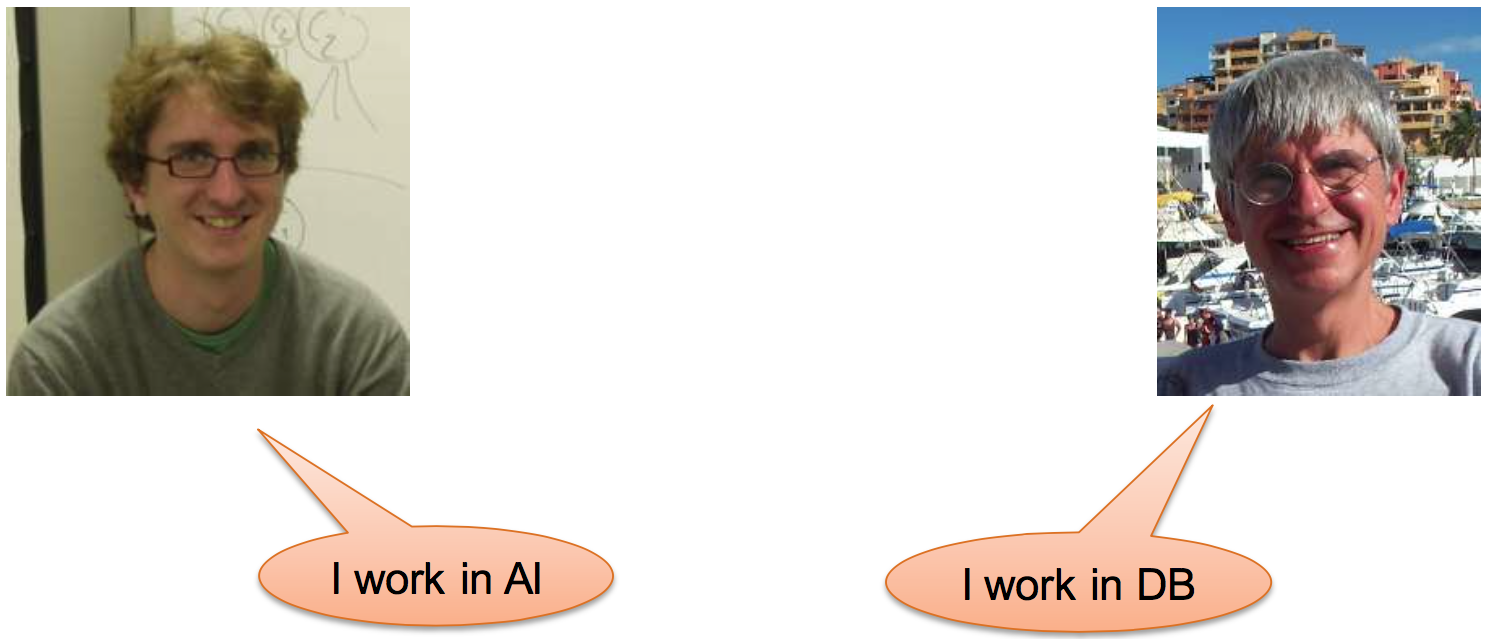
\includegraphics[width=0.91\linewidth]{authors.png}
\end{figure}

\end{frame}

\begin{frame}
\frametitle{Probabilistic Databases}
\bi
\ii \textbf{Data}: standard relational data, plus \myblue{\textit{probabilities}} that measure the degree of uncertainty
\ei
\bi
\ii \textbf{Queries}: standard SQL queries, whose answers are annotated with \myblue{\textit{output probabilities}}
\ei
\end{frame}

%------------------------------------------------

\begin{frame}
\frametitle{A Little History of Probabilistic DBs}
\begin{columns}[c] % The "c" option specifies centered vertical alignment while the "t" option is used for top vertical alignment

\column{.45\textwidth} % Left column and width
\textbf{Early days}
\bi
\ii Wong'82
\ii Shoshani'82
\ii Cavallo\&Pittarelli'87
\ii Barbara'92
\ii Lakshmanan'97,'01
\ii Fuhr\&Roellke'97
\ii Zimanyi'97
\ei
\textbf{Main Challenge:}\\
\mygreen{\textit{Query Evaluation}}\\
(=Probabilistic Inference)

\column{.5\textwidth} % Right column and width
\textbf{Recent work}
\bi
\ii Stanford (Trio)
\ii UW (MystiQ)
\ii Cornell (MayBMS)
\ii Oxford (MayBMS)
\ii U.of Maryland
\ii IBM Almaden (MCDB)
\ii Rice (MCDB)
\ii U. of Waterloo
\ii UBC
\ii U. of Florida
\ii Purdue University
\ii U. of Wisconsin
\ei

\end{columns}
\end{frame}
%------------------------------------------------

\begin{frame}
\frametitle{Why?}
Many applications need to manage \myred{\textit{uncertain data}}
\bi
\ii Information extraction
\ii Knowledge representation
\ii Fuzzy matching
\ii Business intelligence
\ii Data integration
\ii Scientific data management
\ii Data anonymization
\ei
\end{frame}

%------------------------------------------------

\begin{frame}
\frametitle{What?}
\bi
\ii \myblue{Probabilistic Databases} extend Relational Databases with \myred{\textit{probabilities}}

\ii Combine \myblue{Formal Logic} with \myred{Probabilistic Inference}

\ii Requires a new thinking for both databases and probabilistic inference

\ei
\end{frame}

%------------------------------------------------

\begin{frame}
\frametitle{What You Will Learn}
\bi
\ii \textbf{Background:}
\bi
\ii Relational data model: tables, queries, relational algebra
\ii PTIME, NP, \#P
\ii Model counting: DPLL, OBDD, FBDD, d-DNNF
\ei
\ei

\bi
\ii \textbf{In detail:}
\bi
\ii Extensional plans, extensional evaluation, running them in postgres
\ii The landscape of query complexity: from PTIME to  \#P-complete,
\ii Query compilation: Read-Once Formulas, OBDD, FBDD, d-DNNF
\ei
\ei

\bi
\ii \textbf{Less detail:}
\bi
\ii The \#P-hardness proof, complexity of BDDs
\ei
\ei

\bi
\ii \textbf{Omitted:}
\bi
\ii Richer data models: BID, GM, XML, continuous random values)
\ii Approximate query evaluation,
\ii Ranking query answers
\ei
\ei

\end{frame}



\begin{frame}
\frametitle{Outline} % Table of contents slide, comment this block out to remove it
\tableofcontents 
% Throughout your presentation, if you choose to use \section{} and \subsection{} commands, these will automatically be printed on this slide as an overview of your presentation
\end{frame}

%----------------------------------------------------------------------------------------
%	PRESENTATION SLIDES
%----------------------------------------------------------------------------------------


%------------------------------------------------
\section{Motivation} 
%------------------------------------------------

\begin{frame}
\frametitle{Motivation}
\bi
\ii \textbf{Why do we need relational representations of uncertainty?}
\ei

\bi
\ii \textbf{Why do we need lifted inference algorithms?}
\ei
\end{frame}

\begin{frame}
\frametitle{Why Relational Data?}
\bi
\ii \textbf{Our data is already relational!}
\bi
\ii Companies run relational databases
\ii Scientific data is relational:
\bi
\ii Large Hadron Collider generated 25PB in 2012 
\ii LSST Telescope will produce 30TB per night
\ei
\ei
\ei

\bi
\ii \textbf{Big data is big business:}
\bi
\ii Oracle: \$7.1BN in sales
\ii IBM: \$3.2BN in sales
\ii Microsoft: \$2.6BN in sales
\ei
\ei
\end{frame}

%------------------------------------------------
\begin{frame}
\frametitle{Why Relational Data?}
\bi
\ii \textbf{Our data is already relational!}
\bi
\ii Companies run relational databases
\ii Scientific data is relational:
\bi
\ii Large Hadron Collider generated 25PB in 2012 
\ii LSST Telescope will produce 30TB per night
\ei
\ei
\ei

\bi
\ii \textbf{Big data is big business:}
\bi
\ii Oracle: \$7.1BN in sales
\ii IBM: \$3.2BN in sales
\ii Microsoft: \$2.6BN in sales
\ei
\ei
\end{frame}

%------------------------------------------------
\begin{frame}
\frametitle{Why Probabilistic Relational Data?}
\bi
\ii \textbf{Relational data is increasingly probabilistic}
\bi
\ii NELL machine reading ($>$50M tuples)
\ii Google Knowledge Vault ($>$2BN tuples)
\ii DeepDive ($>$7M tuples)
\ei
\ei

\bi
\ii \textbf{Data is inferred from unstructured information using statistical models}
\bi
\ii Learned from the web, large text corpora, ontologies, etc.
\ii The learned/extracted data is relational
\ei
\ei
\end{frame}

%------------------------------------------------
\begin{frame}
\frametitle{Representation: Probabilistic Databases}
\bi
\ii \textbf{Tuple-independent probabilistic databases}
\ei

\begin{figure}[h]
\centering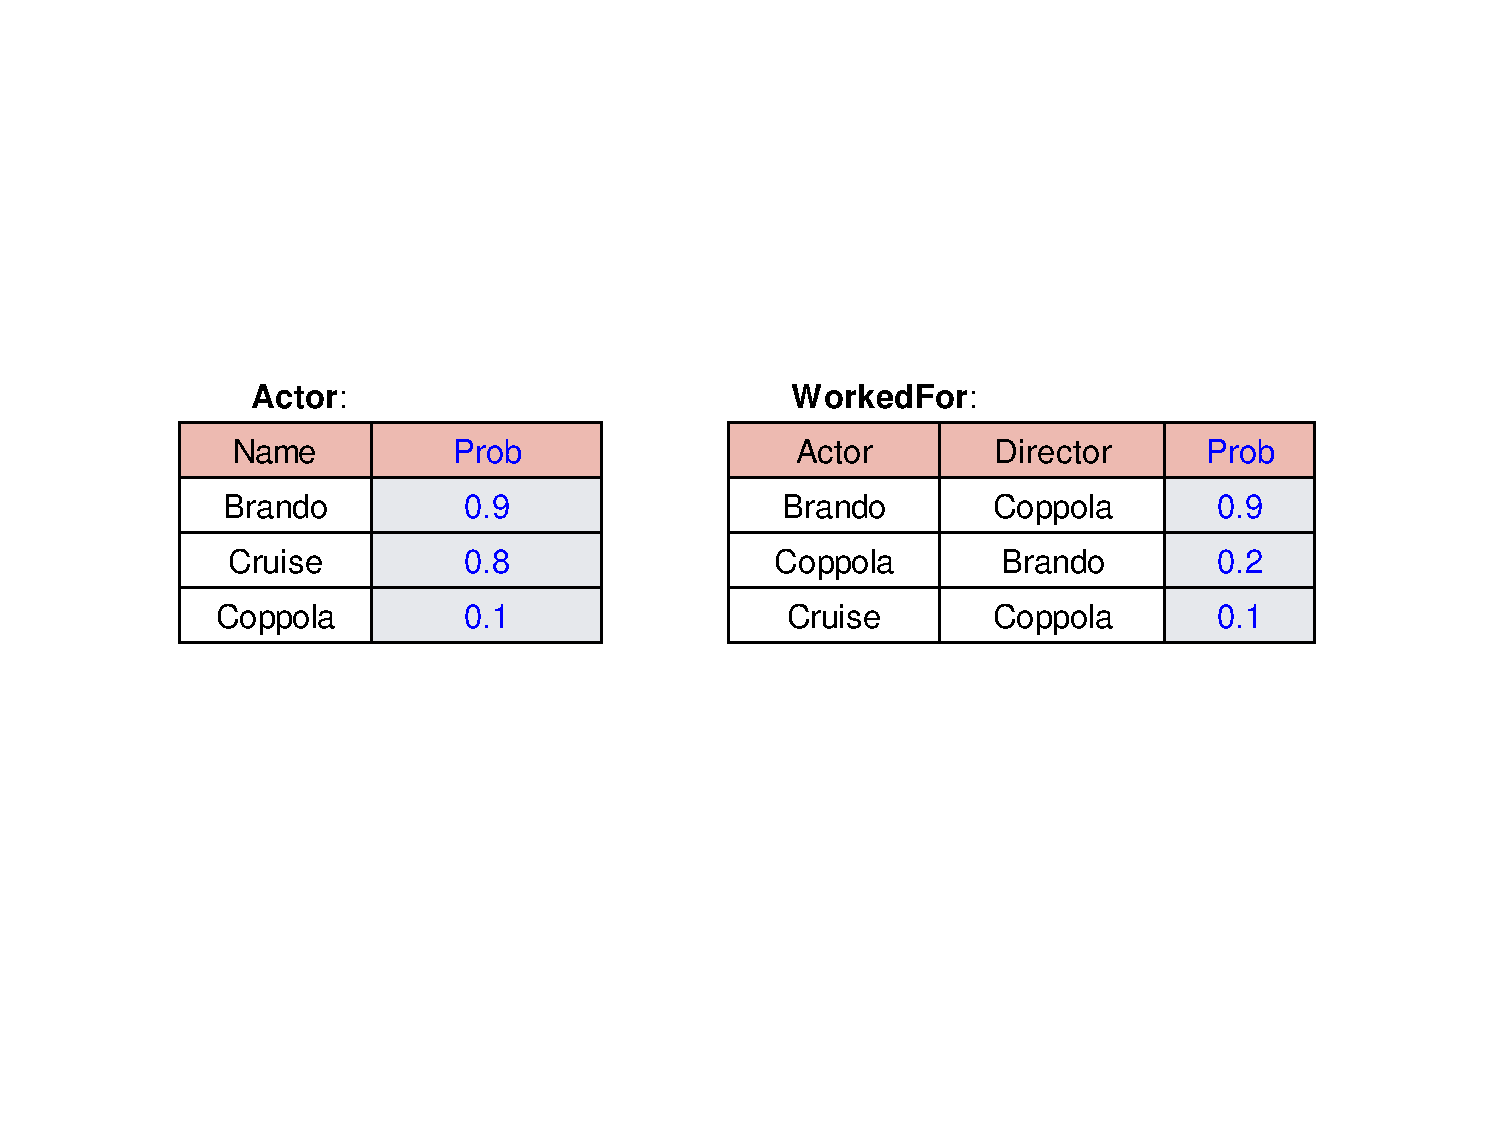
\includegraphics[width=0.91\linewidth]{actor-table.pdf}
\end{figure}

\bi
\ii \textbf{Query: SQL or First Order Logic}
\ei

\begin{figure}[h]
\centering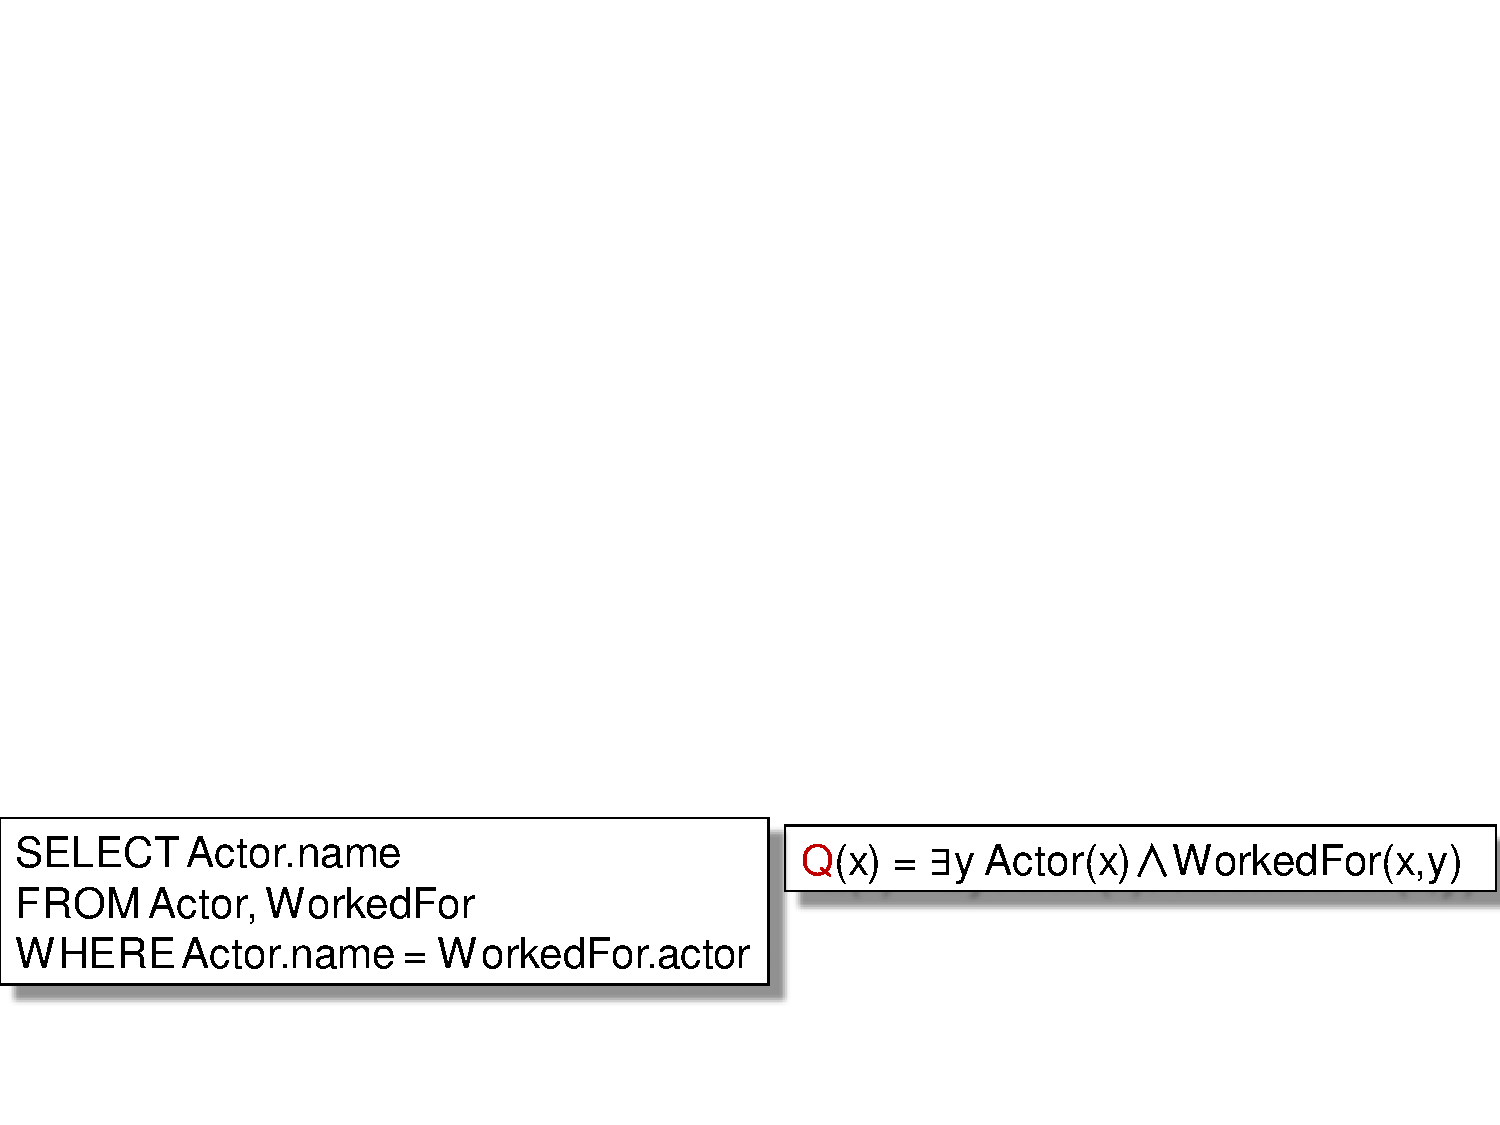
\includegraphics[width=0.91\linewidth]{actor-sql.pdf}
\end{figure}

\end{frame}

%------------------------------------------------
\begin{frame}
\frametitle{Summary}

\begin{figure}[h]
\centering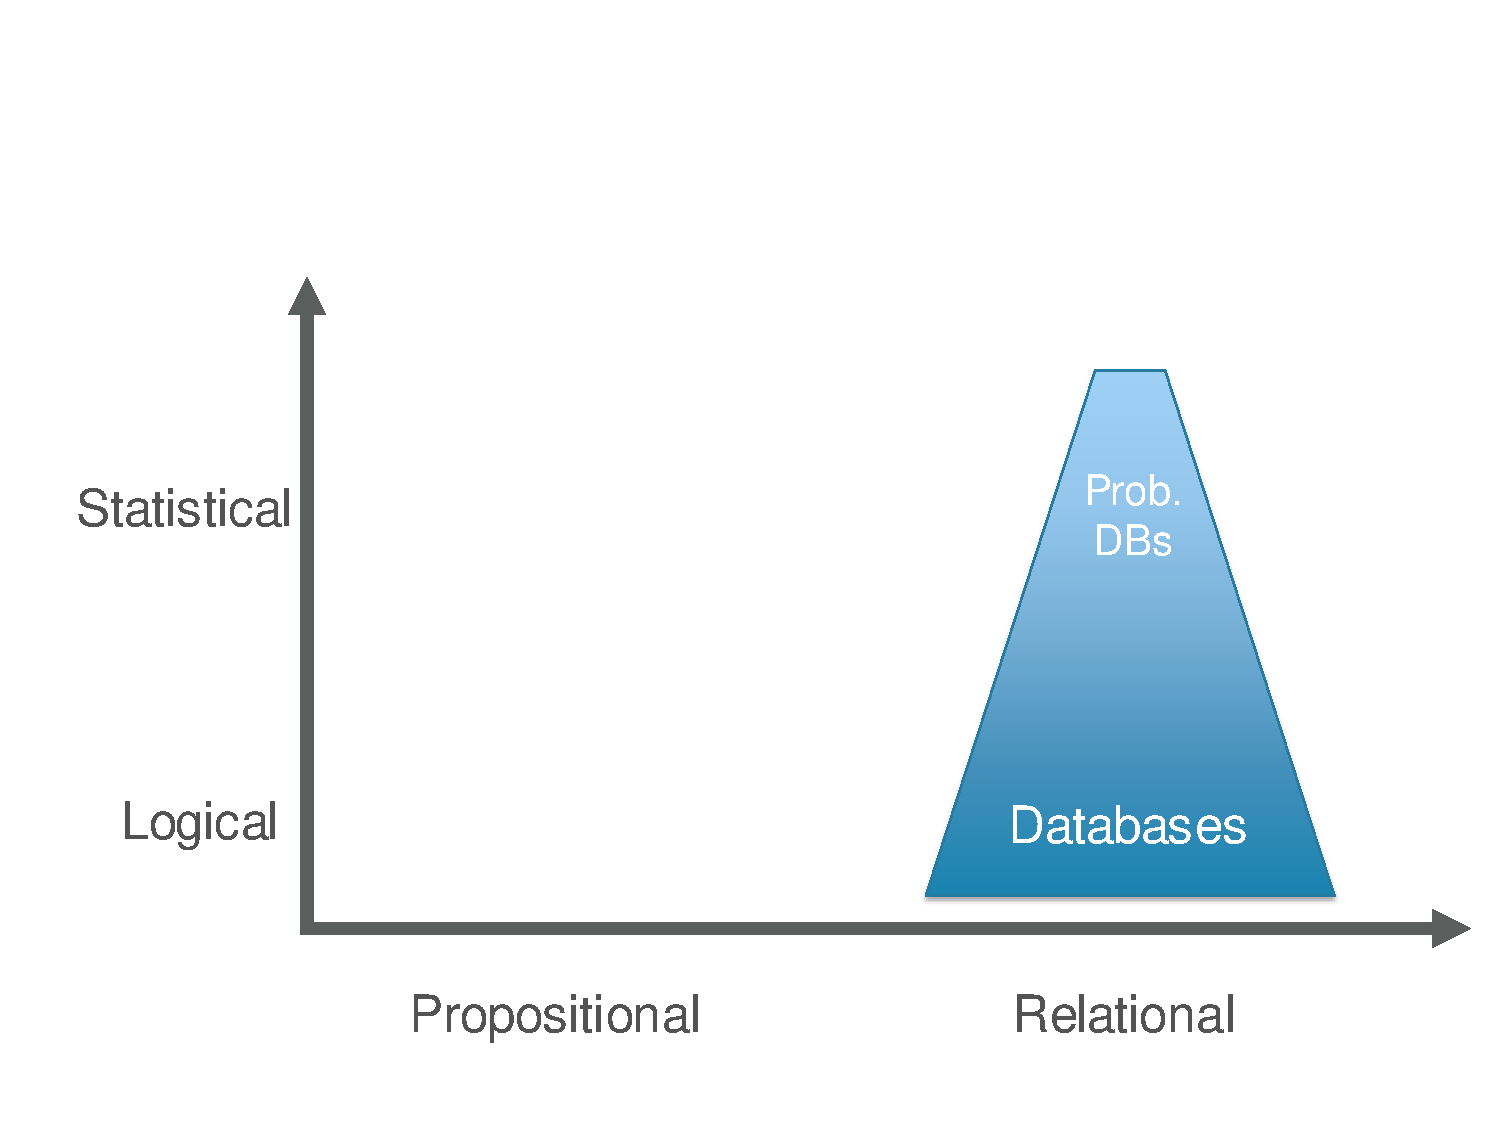
\includegraphics[width=0.95\linewidth]{prob-dbs.pdf}
\end{figure}
\end{frame}

%------------------------------------------------
\begin{frame}
\frametitle{Representations in AI and ML}
\begin{figure}[h]
\centering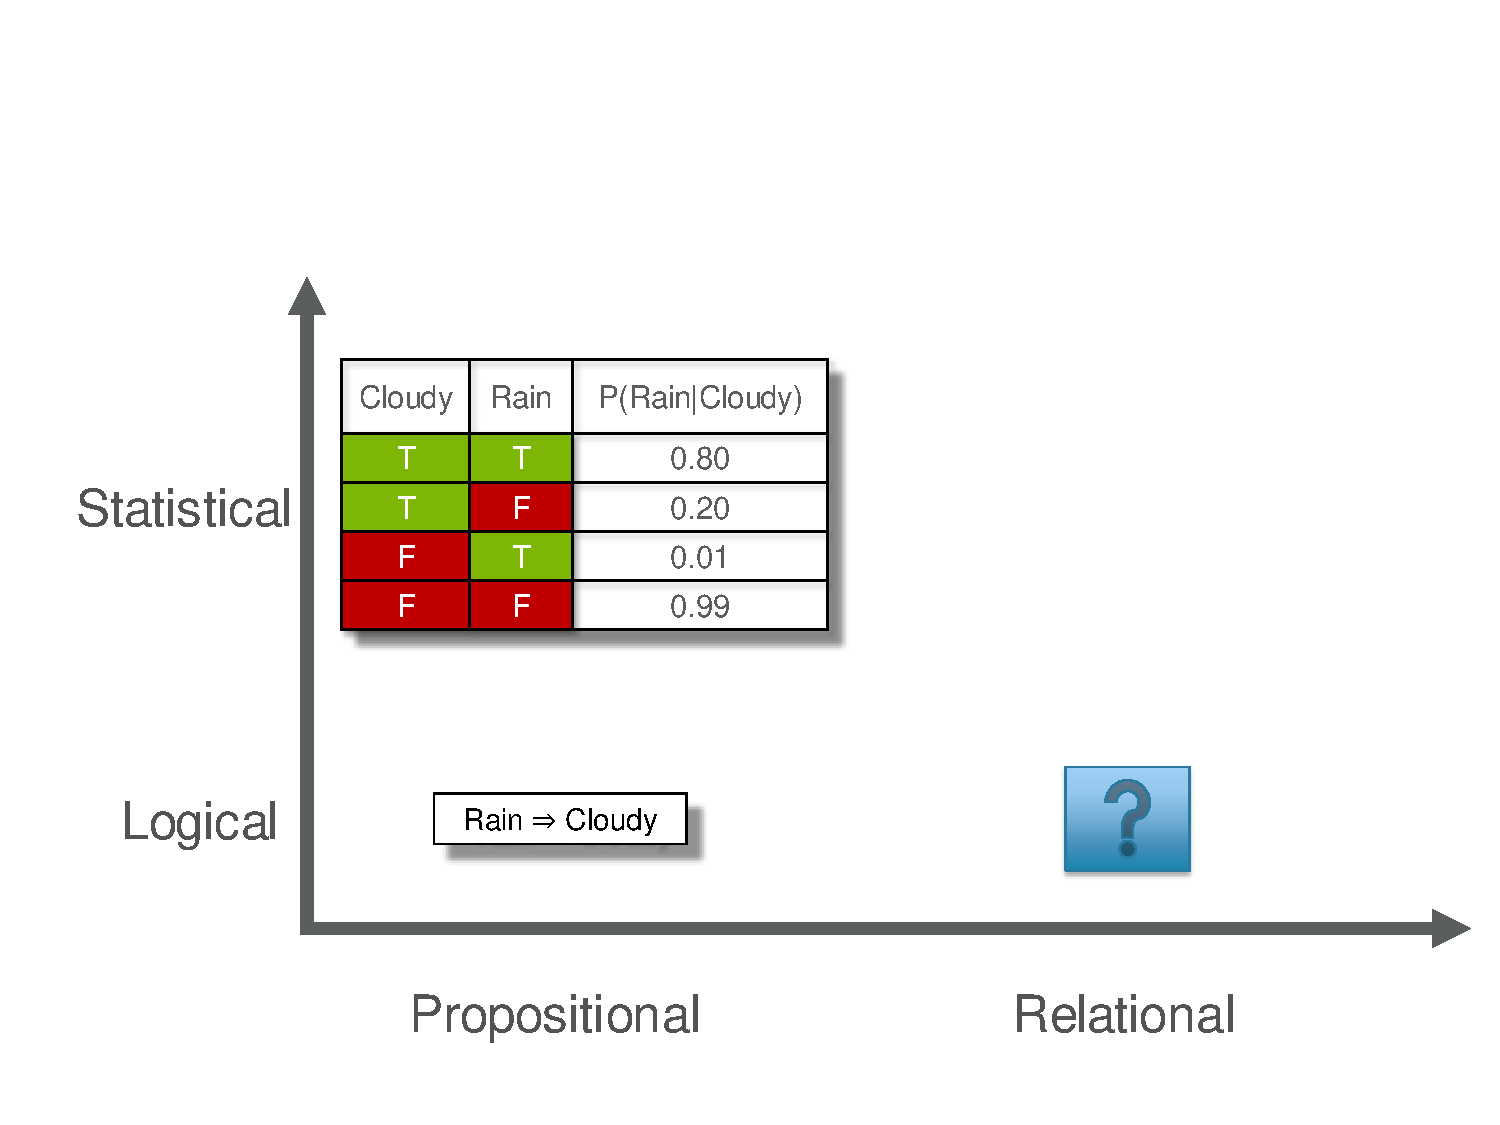
\includegraphics[width=0.95\linewidth]{ai-ml.pdf}
\end{figure}
\end{frame}

%------------------------------------------------
\begin{frame}
\frametitle{Relational Representations}
\bi
\ii Example: First-Order Logic
\ei
\begin{figure}[h]
\centering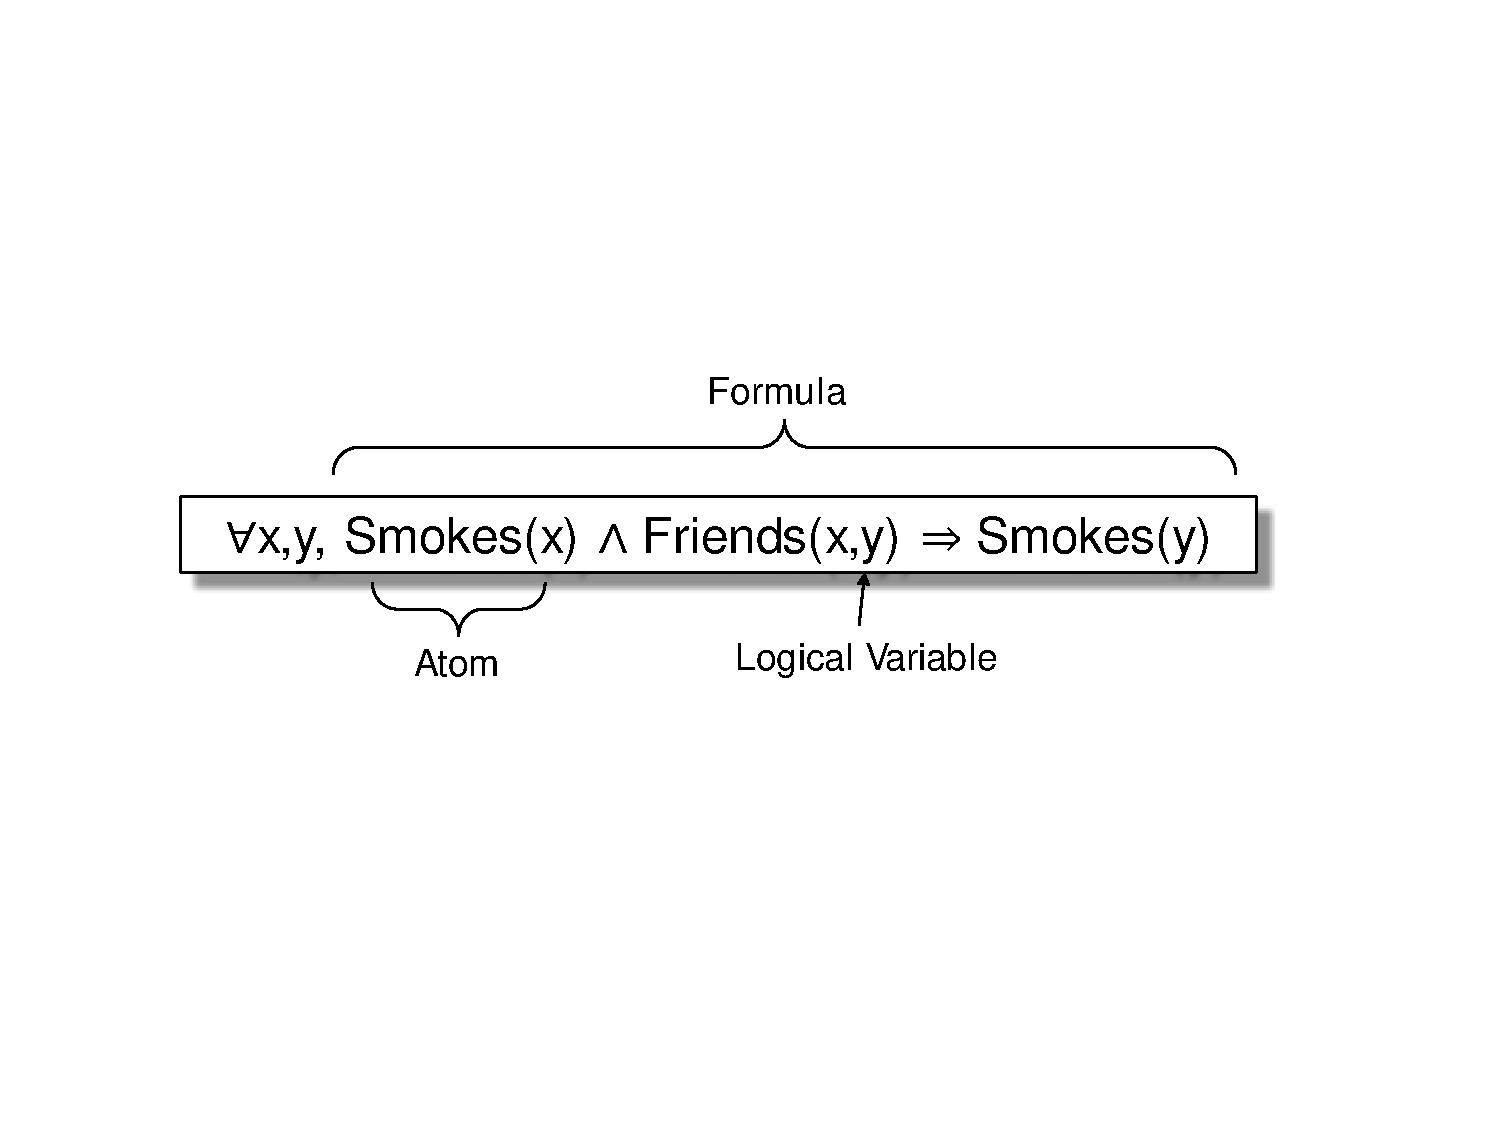
\includegraphics[width=0.75\linewidth]{first-order-logic.pdf}
\end{figure}

\bi
\ii Logical variables have domain of constants \\
x, y range over domain People = \{Alice, Bob\}
\ii Ground formula has no logical variables \\
Smokes(Alice) $\wedge$ Friends(Alice, Bob) $\Rightarrow$ Smokes(Bob)
\ei

\end{frame}

%------------------------------------------------
\begin{frame}
\frametitle{Representations in AI and ML}
\begin{figure}[h]
\centering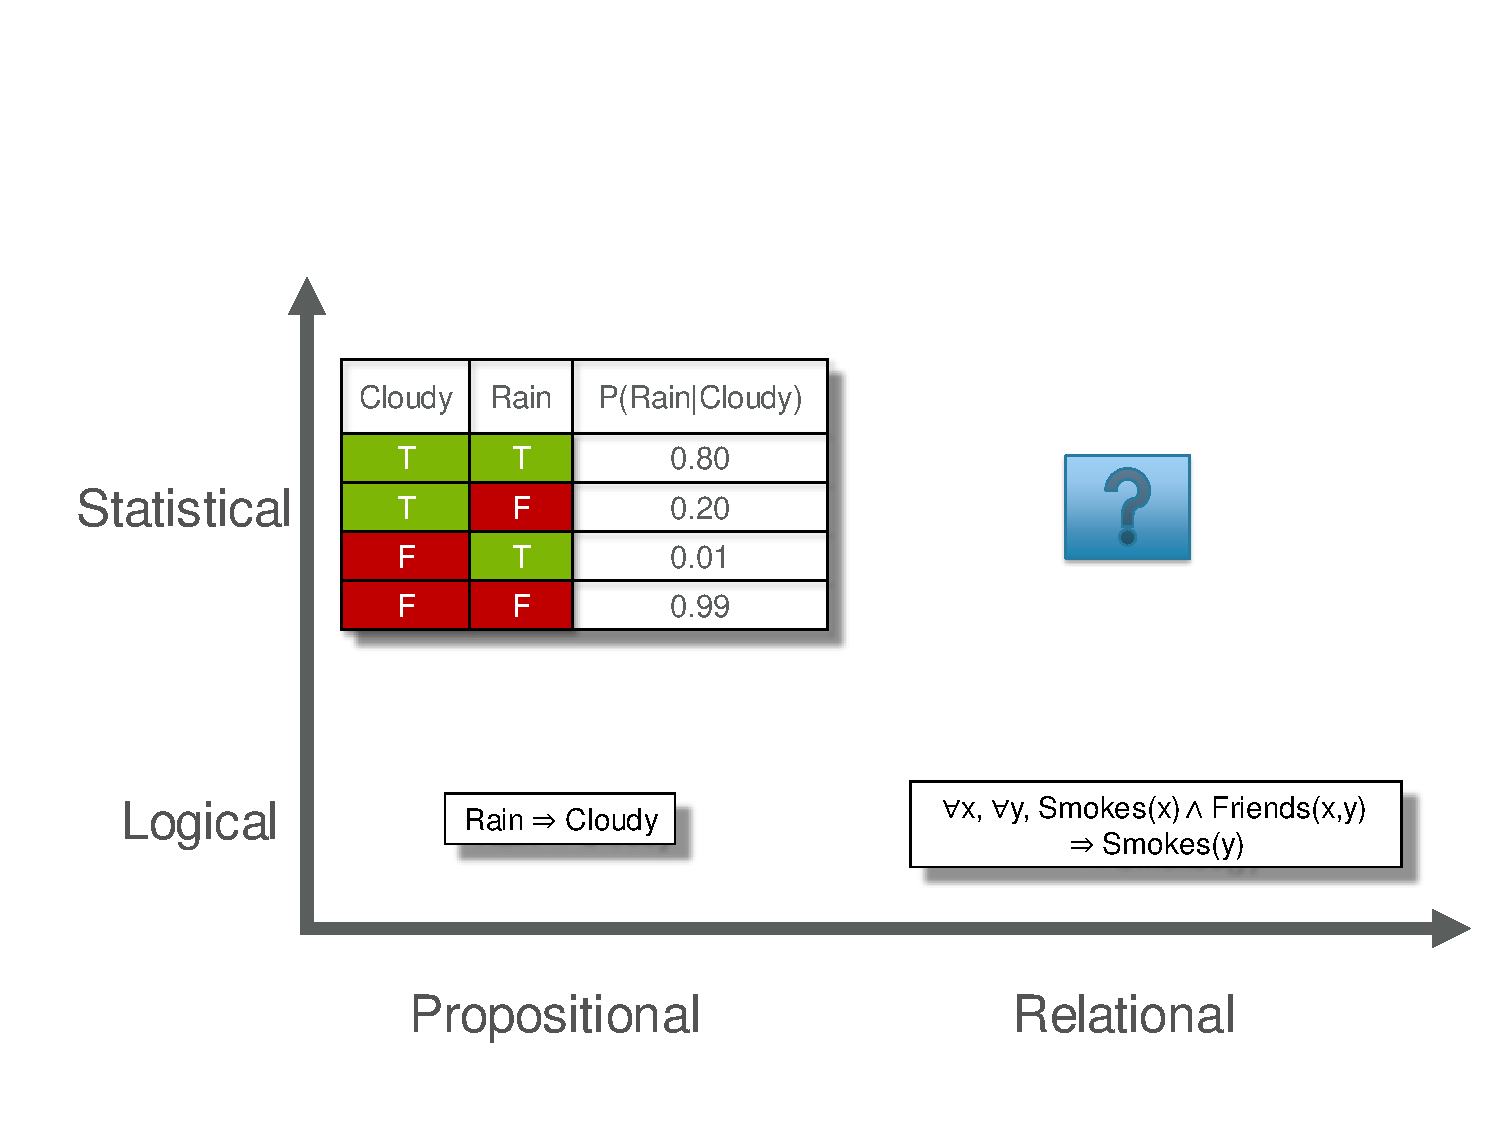
\includegraphics[width=0.95\linewidth]{ai-ml2.pdf}
\end{figure}
\end{frame}

%------------------------------------------------
\begin{frame}
\frametitle{Why Statistical Relational Models?}
\bi
\ii \textbf{Probabilistic graphical models}
\bi
\ii Quantify uncertainty and noise
\ii Not very expressive\\
\textit{Rules of chess in 100,000 pages}
\ei
\ei
\bi
\ii \textbf{First-order logic}
\bi
\ii Very expressive\\
\textit{Rules of chess in 1 page}
\ii Good match for abundant relational data
\ii Hard to express uncertainty and noise
\ei
\ei
\end{frame}

%------------------------------------------------
\begin{frame}
\frametitle{Example: Markov Logic}
\bi
\ii \textbf{Weighted First-Order Logic}
\ei
\begin{figure}[h]
\centering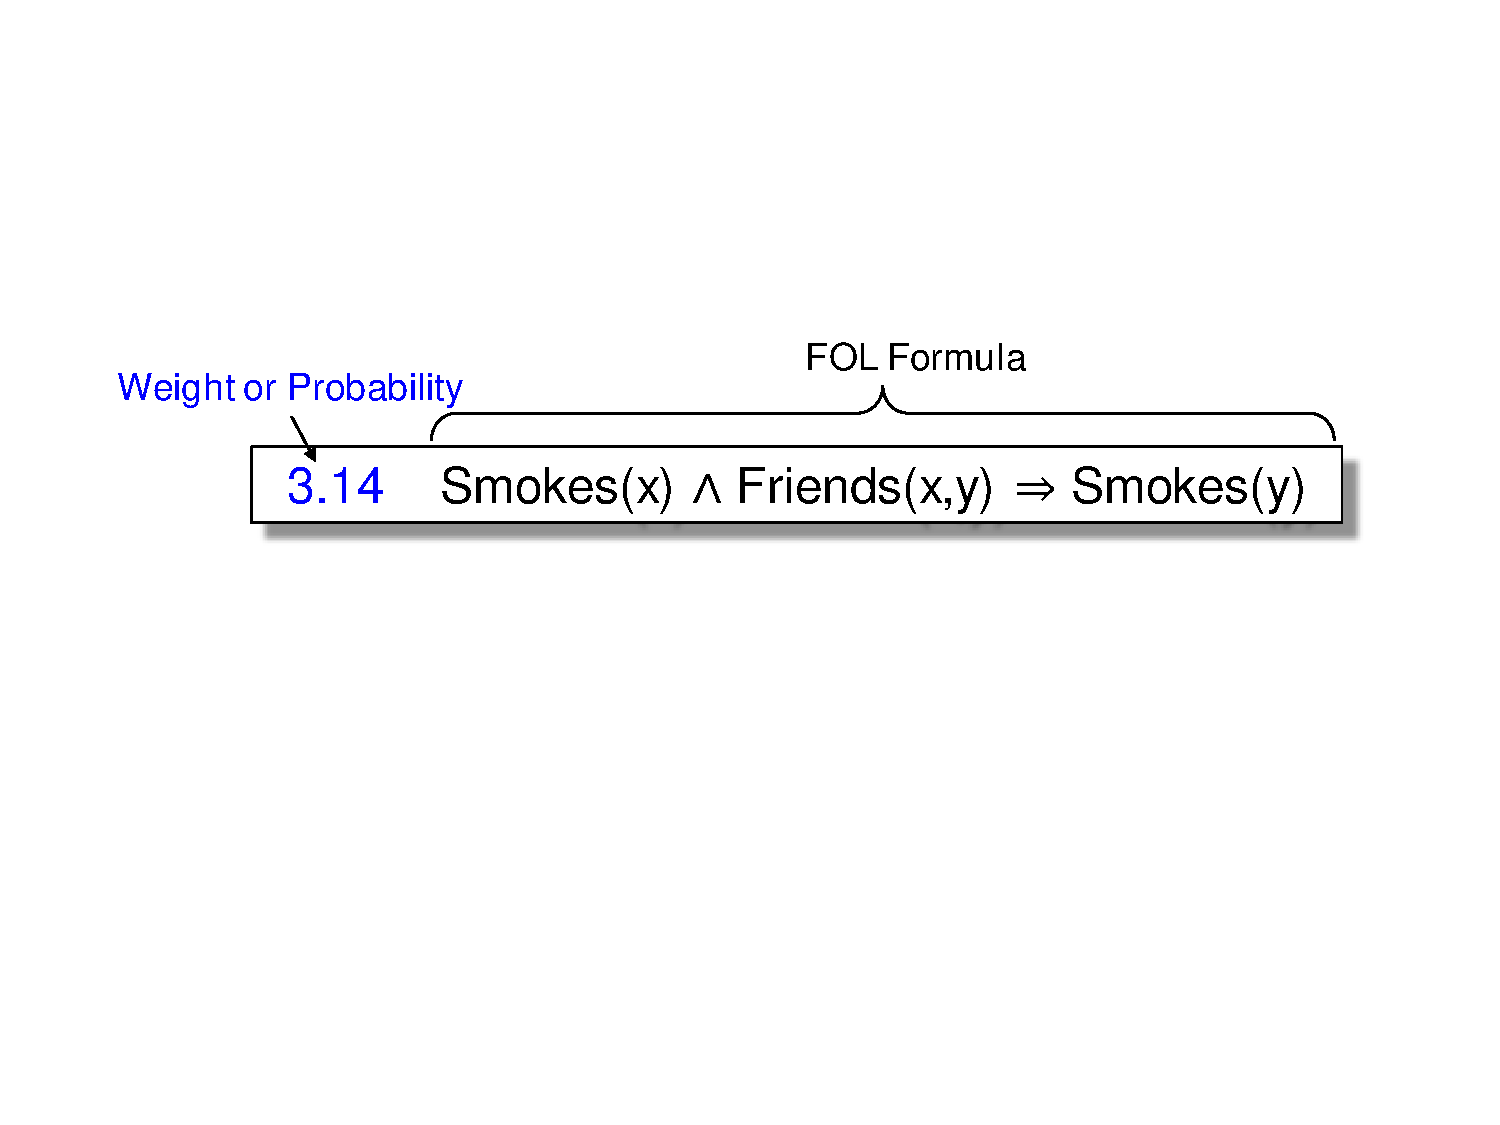
\includegraphics[width=0.75\linewidth]{probability.pdf}
\end{figure}

\bi
\ii \textbf{Ground atom/tuple = \myblue{random variable} in \{true, false\}}\\
e.g., Smokes(Alice), Friends(Alice, Bob), etc
\ii \textbf{Ground atom/tuple = \myred{factor} in propositional factor graph}
\ei

\begin{figure}[h]
\centering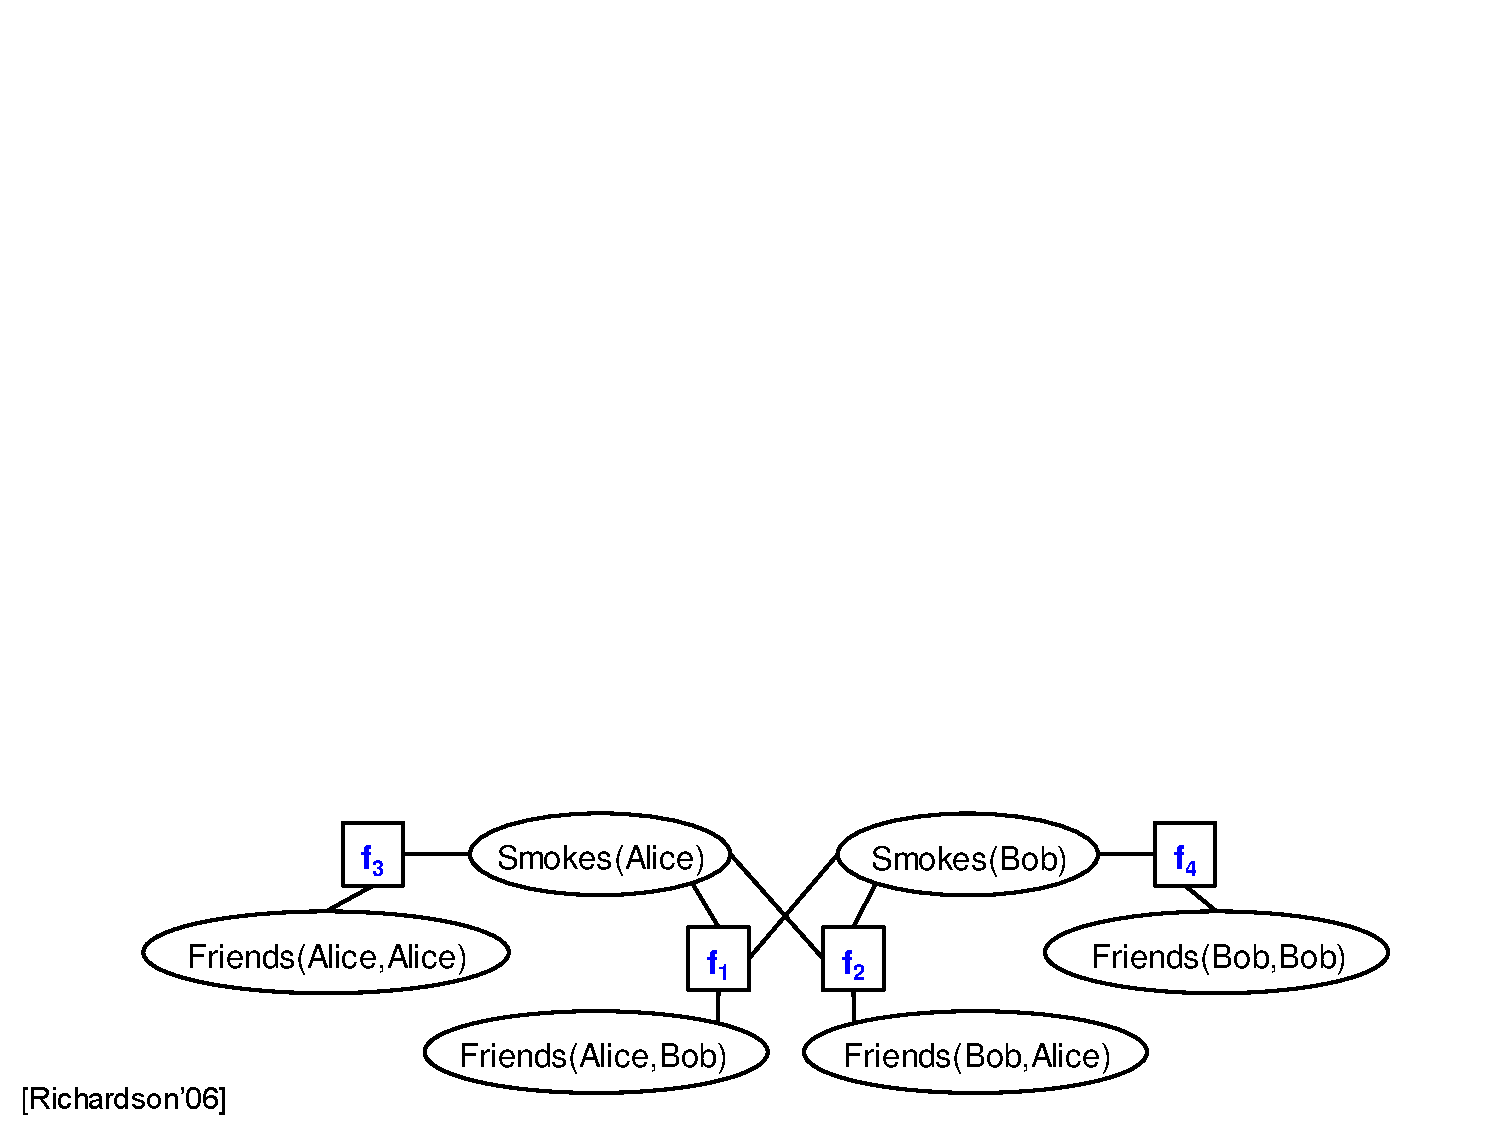
\includegraphics[width=0.75\linewidth]{richardson.pdf}
\end{figure}

\end{frame}

%------------------------------------------------
\begin{frame}
\frametitle{Representations in AI and ML}
\begin{figure}[h]
\centering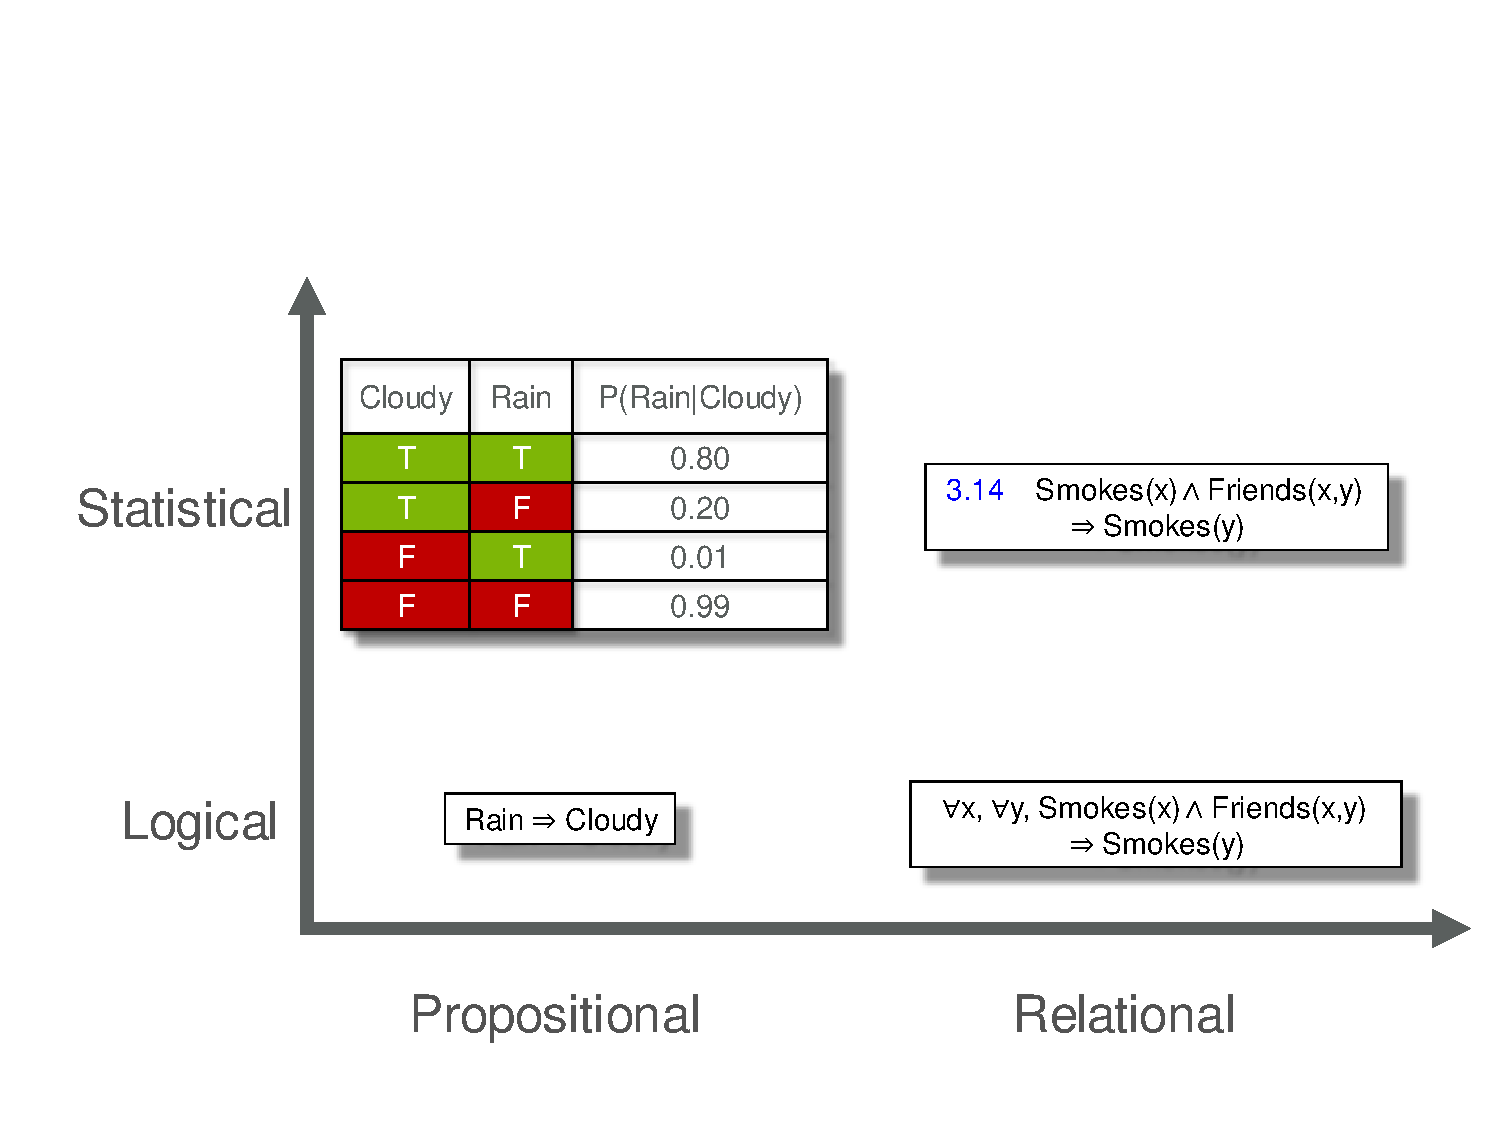
\includegraphics[width=0.95\linewidth]{ai-ml3.pdf}
\end{figure}
\end{frame}

%------------------------------------------------
\begin{frame}
\frametitle{Representations in AI and ML}
\begin{figure}[h]
\centering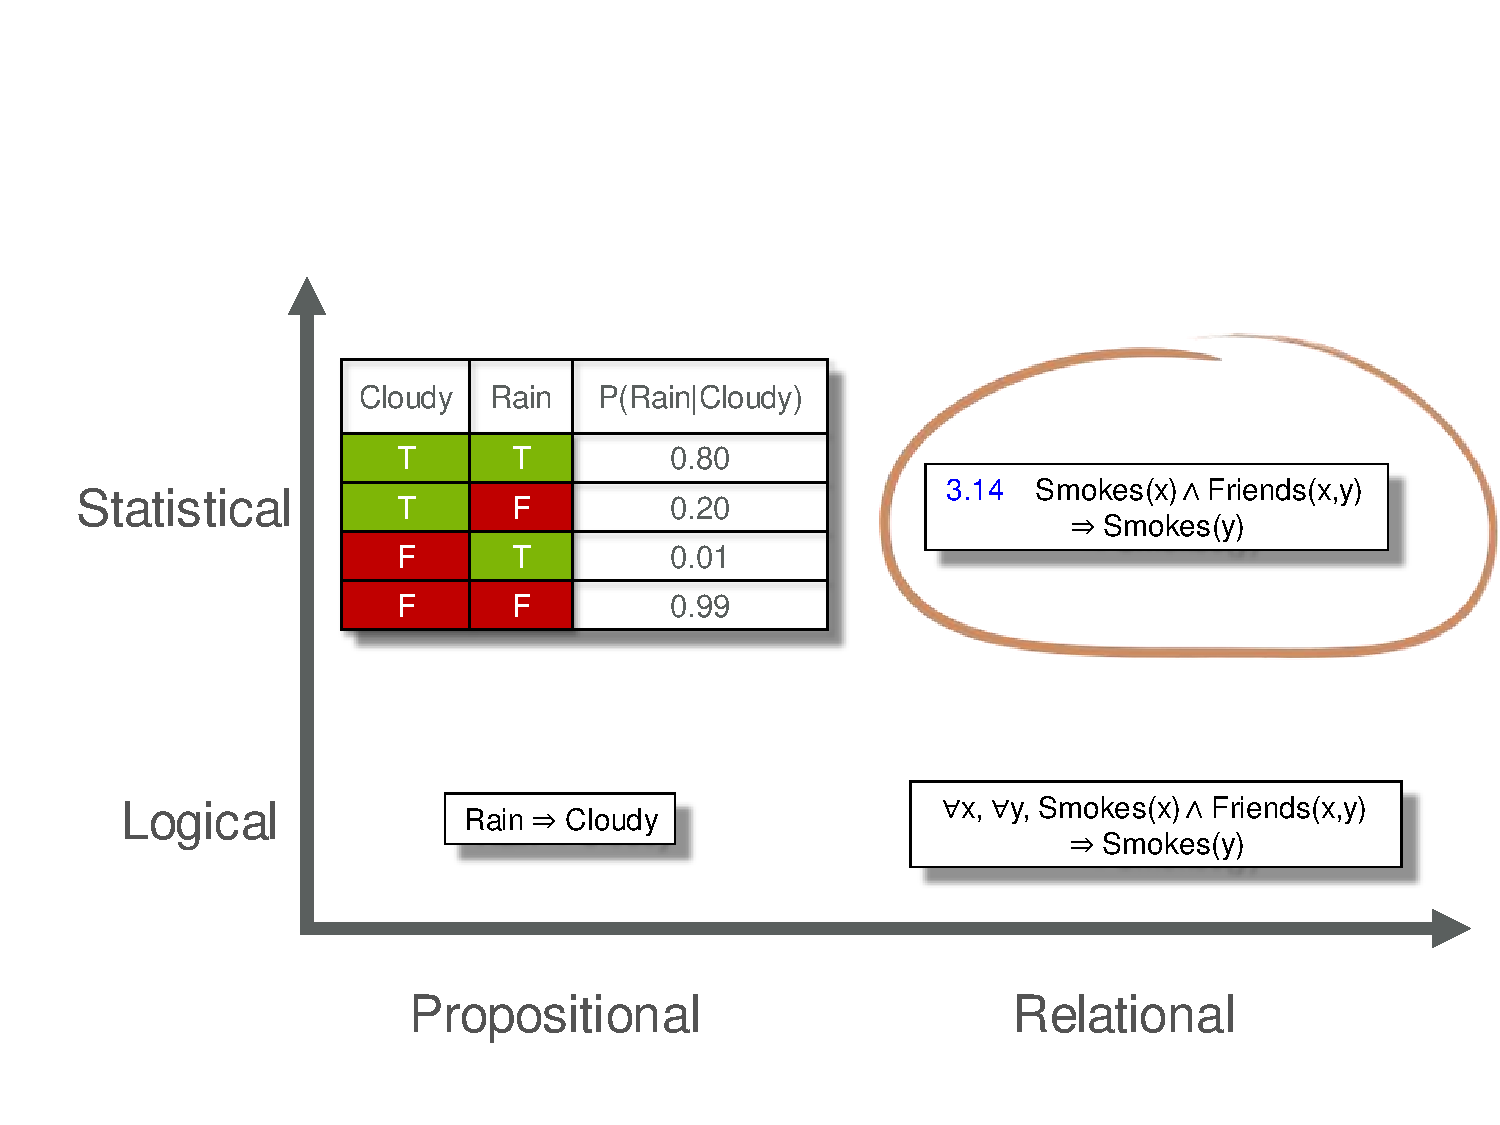
\includegraphics[width=0.95\linewidth]{ai-ml4.pdf}
\end{figure}
\end{frame}

%------------------------------------------------
\begin{frame}
\frametitle{Summary}
\begin{figure}[h]
\centering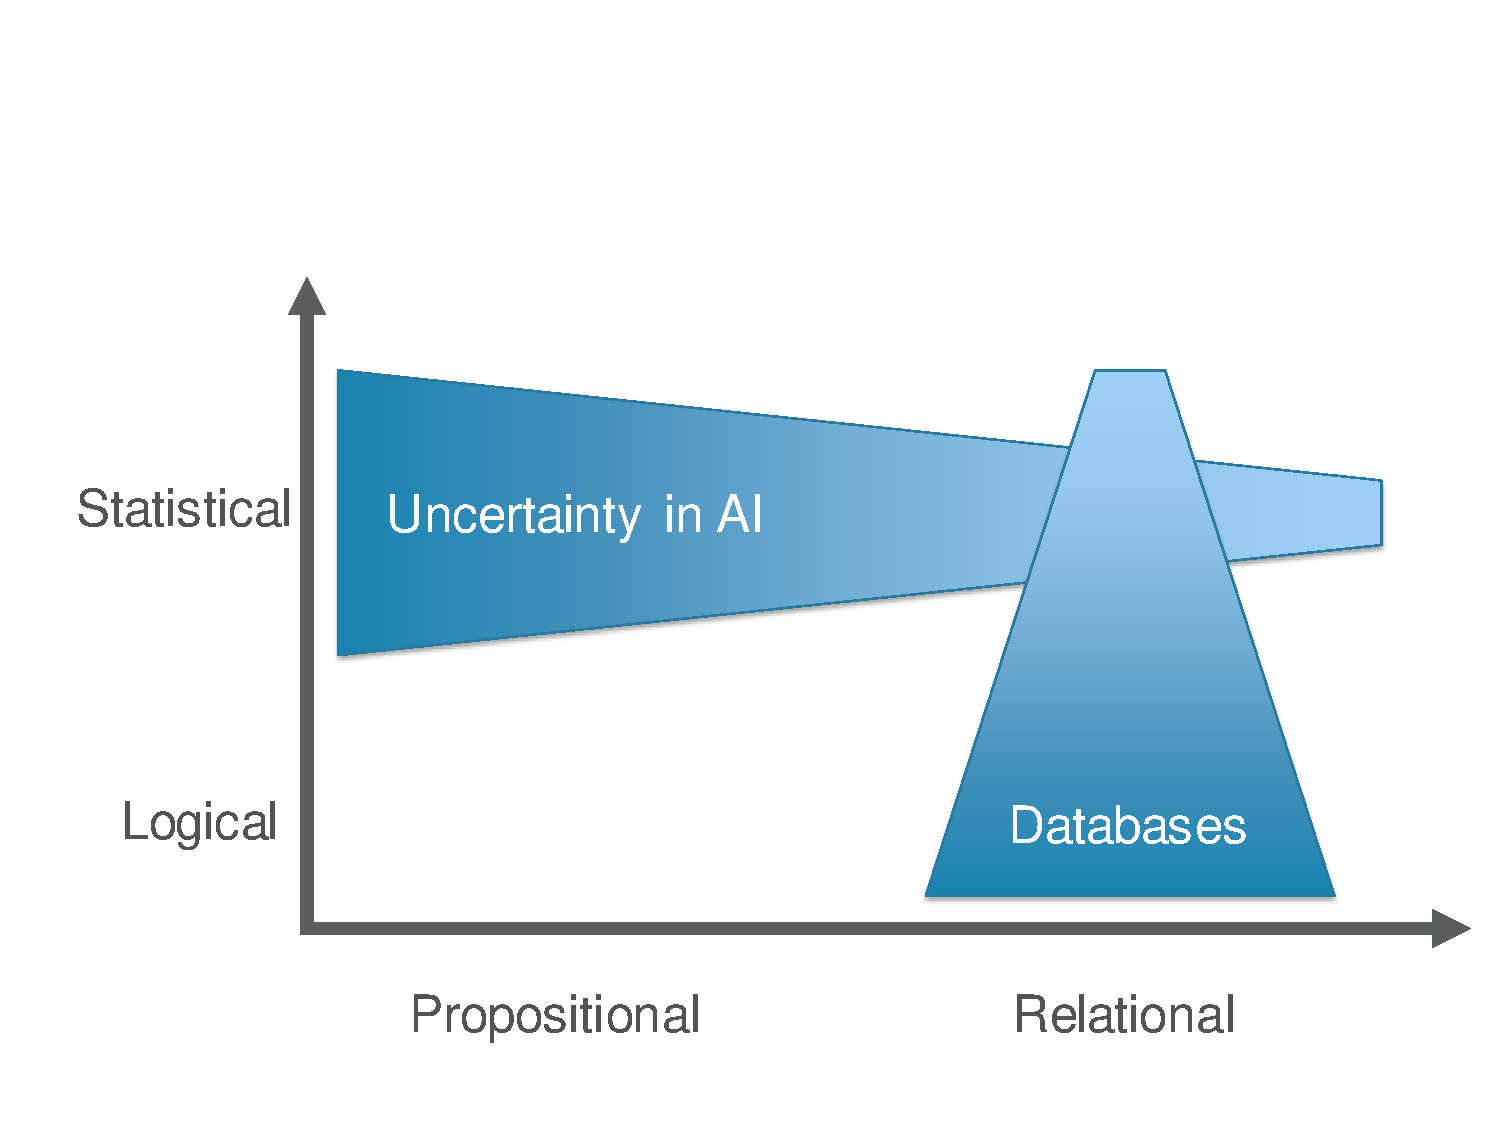
\includegraphics[width=0.95\linewidth]{summary1.pdf}
\end{figure}
\end{frame}

%------------------------------------------------
\begin{frame}
\frametitle{Summary}
\begin{figure}[h]
\centering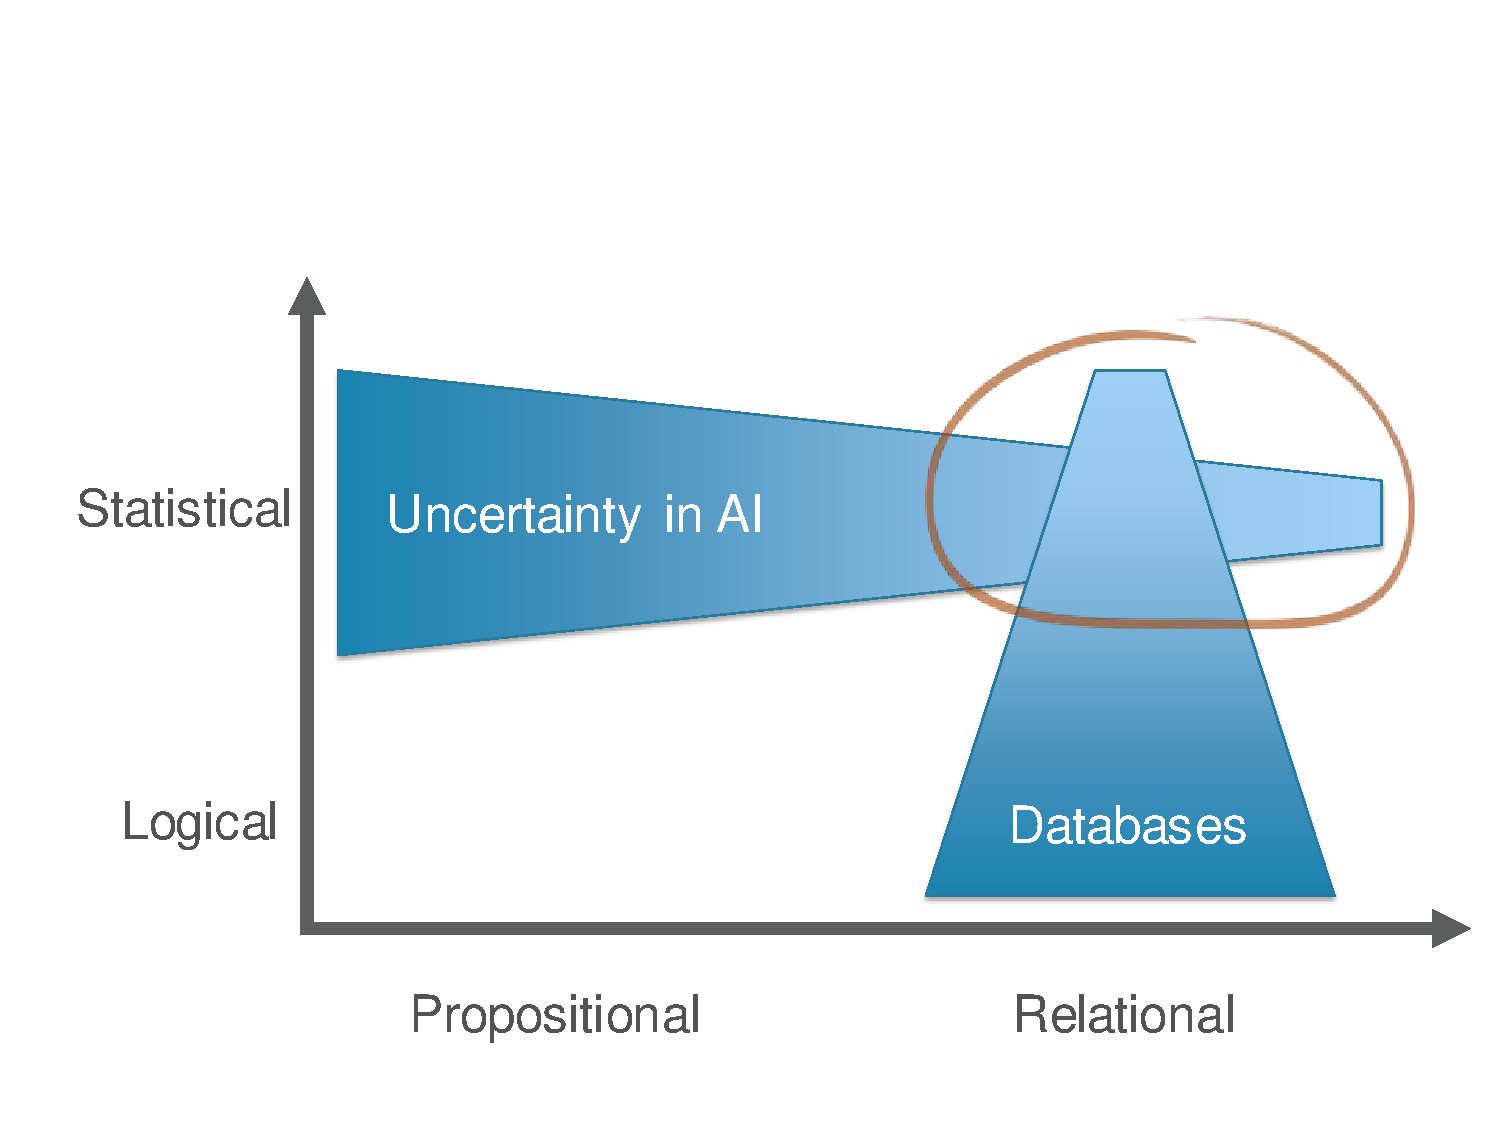
\includegraphics[width=0.95\linewidth]{summary2.pdf}
\end{figure}
\end{frame}

%------------------------------------------------
%\begin{frame}
%\frametitle{Title}
%
%\end{frame}

\end{document} 